\documentclass[letterpaper, 10pt, journal]{IEEEtran}
\usepackage{graphicx}
\usepackage{float}
\usepackage{listings}
\usepackage{color}
\usepackage{multirow}
\usepackage[table,xcdraw]{xcolor}
\usepackage[justification=centering]{caption}

\graphicspath{ {./Images/} }

\lstset{frame=tb,
  language=Java,
  aboveskip=3mm,
  belowskip=3mm,
  showstringspaces=false,
  columns=flexible,
  basicstyle={\small\ttfamily},
  numbers=none,
  numberstyle=\tiny\color{gray},
  keywordstyle=\color{blue},
  commentstyle=\color{dkgreen},
  stringstyle=\color{mauve},
  breaklines=true,
  breakatwhitespace=true,
  tabsize=3
}

\begin{document}
\title{Tarea 1 - Reporte de \LaTeX}
\author{Kathy~Brenes~Guerrero, Barnum~Castillo~Barquero

~\IEEEmembership{
    \begin{center}
        Maestr\'ia en Ciencias de la Computaci\'on, Introducci\'on a la Investigaci\'on, ITCR
    \end{center}
}}% <-this % stops a space

% The paper headers
\markboth{Instituto Tecnol\'ogico de Costa Rica, Introducci\'on a la Investigaci\'on, Agosto~2018}%
{Shell \MakeLowercase{\textit{et al.}}: Tarea 1 - Reporte de \LaTeX}
\maketitle

\begin{abstract}
One of the biggest issues that an operating system can experience is privilege escalation. Privilege escalation is the act of exploiting a bug, design flaw, or configuration oversight in an operating system or software application to gain elevated access to resources that are normally protected from an application or user. Understanding the weaknesses and flaws of a security level issue for the operating system can help implement better approaches and techniques to improve the software itself. Just because you have updated your computer to the latest update or patch, doesn’t mean that it has been secured. Windows, for example, has a series of vulnerabilities that can affect the operating system and can't be solved by Microsoft because the updates can create incompatibilities with an older system or with some security protocols. The Privilege Escalation technique takes advantage of these vulnerabilities to  gain privileges (access) within a remote  system, in order to run applications and make commands on it. The focus of this paper is to list the vulnerabilities that have been demonstrated by third party systems in different operating system, and provide a technical point of view  on what can be done to avoid these breaches ( vulnerabilities or impacts). An Operation System breach can enable attackers to increase their level of control over target systems, such that they are free to access any data or make any configuration changes\cite{Williams}. This study reveals the importance of the way in which current systems should be defended from this mechanism.
\end{abstract}
\begin{IEEEkeywords}
Operating System, Penetration Testing, Cybersecurity, Internet of Things.
\end{IEEEkeywords}

\section{Introduction}
To start talking about vulnerabilities, it might be easier to start with past operating systems, specifically MS-DOS and Windows 9x (95, 98 and Me), which were based on MS-DOS.
All software running on an MS-DOS-based system was treated equally. Any program could, literally, do anything. Any program could play directly with the hardware, poke around in memory being used by other programs, or even modify the operating system itself on the fly.

It was not what we\'’d call \'“secure\'” in any way. We suppose the only thing that prevented it from being a security nightmare is that today’s ubiquitous connectivity didn\'’t exist. Compared to what we take for granted today, it was at least cumbersome, and often outright difficult, to get data from one computer to another. Since the kernel can do anything, we refer to it as having more privilege than software running in user-mode. There are a number of different things that can be restricted based on privilege, but memory access is one of the clearer examples

A program running user-mode cannot read and write the memory of another program that happens to be running at the same time. Your web browser, for example, is not able to peek into the document you’re currently editing in a word processor.

It’s important to understand that this concept of “privilege escalation” matters. Hopefully, understanding the concept — even at a high level and perhaps only partially — will give you some idea that it’s important, why it’s important, and how it relates to the security of your computer.

Knowing that it’s important, the single most important thing you can do to avoid issues and vulnerabilities that might be characterized as “privilege escalation” issues is to keep your system as up-to-date as possible. As with the recent CPU issue, operating system vendors are quickly putting out patches to avoid it, and it’ll be important for you to have those patches when they come up.

The best way to do that is to keep whatever OS you run — set to update automatically.Being always aware that keeping the operating system updated helps reduce the risk of these attacks but does not eradicate them 100%.

\section{Historia del \LaTeX}


\section{Usos acad\'emicos, extensi\'on, importancia}
Text here ...

\subsection{SubSection 1...}
Text here..
\begin{enumerate}
\item	Some Windows services are configured to run under the Local System user account. A vulnerability such as a buffer overflow (an anomaly where a program, while writing data to a buffer, overruns the buffer\''s boundary and overwrites adjacent memory locations) may be used to execute arbitrary code with privilege elevated to Local System. Alternatively, a system service that is impersonating a lesser user can elevate that user\''s privileges if errors are not handled correctly while the user is being impersonated (e.g. if the user has introduced a malicious error handler)\cite{[6]}.
\item	Under some legacy versions of the Microsoft Windows operating system, the All Users screen saver runs under the Local System account – any account that can replace the current screen saver binary in the file system or Registry can therefore elevate privileges \cite{[6]}.
\item	In certain versions of the Linux kernel it was possible to write a program that would set its current directory to /etc/cron.d, request that a core dump be performed in case it crashes and then have itself killed by another process. The core dump file would have been placed at the program\''s current directory, that is, /etc/cron.d, and cron would have treated it as a text file instructing it to run programs on schedule. Because the contents of the file would be under attacker’s control, the attacker would be able to execute any program with root privileges \cite{[3]}.
\end{enumerate}
Text Here

\section{Estilos de documento}
Text Here
\subsection{Subsection 1}
Example...
\lstset{language=Java}
\begin{lstlisting}
uname -a
cat /proc/version
cat /etc/issue
\end{lstlisting}

\subsection{Subsection 2}
Text here...
\begin{enumerate}
\item Check which processes are running
\lstset{language=Java}
\begin{lstlisting}
# Metasploit
ps
# Linux
ps aux
\end{lstlisting}
\end{enumerate}


\section{C\'omo hacer: p\'arrafos, efectos de letra, tildes, t\'itulos, subt\'itulos, referencias, marcas de agua, headers y footers, manejo de saltos de p\'agina, columnas de la p\'agina, etc.}
\subsection{Subsection 1}
Text here..

\section{Manejo de Tablas}
\subsection{Tabla B\'asica}
Texto
\begin{table}[H]\centering
\begin{tabular}{|l c|r|}
\hline
Columna 1 & Columna 2 & Columna 3 \\ \hline
Fila 11   & Fila 12   & Fila 13   \\ \hline
Fila 21   & Fila 22   & Fila 23   \\ \hline
\end{tabular}
\end{table}

Texto
\lstset{language=Java}
\begin{lstlisting}
\begin{table}[H]\centering
\begin{tabular}{|l c|r|}
\hline
Columna 1 & Columna 2 & Columna 3 \\ \hline
Fila 11   & Fila 12   & Fila 13   \\ \hline
Fila 21   & Fila 22   & Fila 23   \\ \hline
\end{tabular}
\end{table}
\end{lstlisting}

\subsection{Agregar columnas y filas}

Texto
\lstset{language=Java}
\begin{lstlisting}
\begin{table}[H]\centering
\begin{tabular}{|l|l|l|l|}
\hline
Columna 1  & Columna 2 & Columna 3 & C.Nueva \\ \hline
Fila 11    & Fila 12   & Fila 13   & \\ \hline
Fila 21    & Fila 22   & Fila 23   & \\ \hline
Nueva fila &           &           & \\ \hline
\end{tabular}
\end{table}
\end{lstlisting}

Texto
\begin{table}[H]\centering
\begin{tabular}{|l|l|l|l|}
\hline
Columna 1  & Columna 2 & Columna 3 & C.Nueva \\ \hline
Fila 11    & Fila 12   & Fila 13   & \\ \hline
Fila 21    & Fila 22   & Fila 23   & \\ \hline
Nueva fila &           &           & \\ \hline
\end{tabular}
\end{table}

\subsection{M\'utiples columnas}

Texto

\lstset{language=Java}
\begin{lstlisting}
\multicolumn{ancho}{alineamiento}{contenido}
\end{lstlisting}

Texto 
\begin{table}[H]\centering
\begin{tabular}{|l|l|l|}
\hline
Columna 1 & Columna 2  & Columna 3 \\ \hline
\multicolumn{2}{|l|}{Fila 11 + fila 12} & Fila 13 \\ \hline
Fila 21   & Fila 22    & Fila 23   \\ \hline
\end{tabular}
\end{table}

texto

\lstset{language=Java}
\begin{lstlisting}
\begin{table}[H]\centering
\begin{tabular}{|l|l|l|}
\hline
Columna 1 & Columna 2 & Columna 3 \\ \hline
\multicolumn{2}{|l|}{Fila 11 + fila 12} & Fila 13 \\ \hline
Fila 21   & Fila 22   & Fila 23   \\ \hline
\end{tabular}
\end{table}
\end{lstlisting}
Texto
\subsection{M\'utiples filas}
Texto

\lstset{language=Java}
\begin{lstlisting}
\usepackage{multirow}
\end{lstlisting}

La siguiente tabla muestra su uso.
\begin{table}[H]\centering
\begin{tabular}{|l|l|l|}
\hline
Columna 1                & Columna 2 & Columna 3 \\ \hline
\multirow{2}{*}{Fila 11 + fila 21} & Fila 12   & Fila 13   \\ \cline{2-3} 
                         & Fila 22   & Fila 23   \\ \hline
\end{tabular}
\end{table}

\lstset{language=Java}
\begin{lstlisting}
\begin{table}[H]\centering
\begin{tabular}{|l|l|l|}
\hline
Columna 1                & Columna 2 & Columna 3 \\ \hline
\multirow{2}{*}{Fila 11 + fila 21} & Fila 12   & Fila 13   \\ \cline{2-3} 
                         & Fila 22   & Fila 23   \\ \hline
\end{tabular}
\end{table}
\end{lstlisting}

Texto

\subsection{Colores celdas}

\lstset{language=Java}
\begin{lstlisting}
\begin{table}[H]\centering
\begin{tabular}{|l|l|l|}
\hline
\rowcolor[HTML]{FFCE93} 
Columna 1                       & Columna 2 & Columna 3 \\ \hline
\cellcolor[HTML]{3166FF}Fila 11 & Fila 12   & Fila 13   \\ \hline
Fila 21                         & Fila 22   & Fila 23   \\ \hline
\end{tabular}
\end{table}
\end{lstlisting}

\begin{table}[H]\centering
\begin{tabular}{|l|l|l|}
\hline
\rowcolor[HTML]{FFCE93} 
Columna 1                       & Columna 2 & Columna 3 \\ \hline
\cellcolor[HTML]{3166FF}Fila 11 & Fila 12   & Fila 13   \\ \hline
Fila 21                         & Fila 22   & Fila 23   \\ \hline
\end{tabular}
\end{table}

\section{Manejo de figuras y gr\'aficos}
\subsection{Directorio de im\'agenes}
\lstset{language=Java}
\begin{lstlisting}
%Ruta relativa al archivo .tex 
\graphicspath{ {./images/} }

%Ruta absoluta
\graphicspath{ {c:/user/images/} }
\end{lstlisting}

\subsection{Modificar tama\~no y rotaci\'on}
Text here.\\

\lstset{language=Java}
\begin{lstlisting}
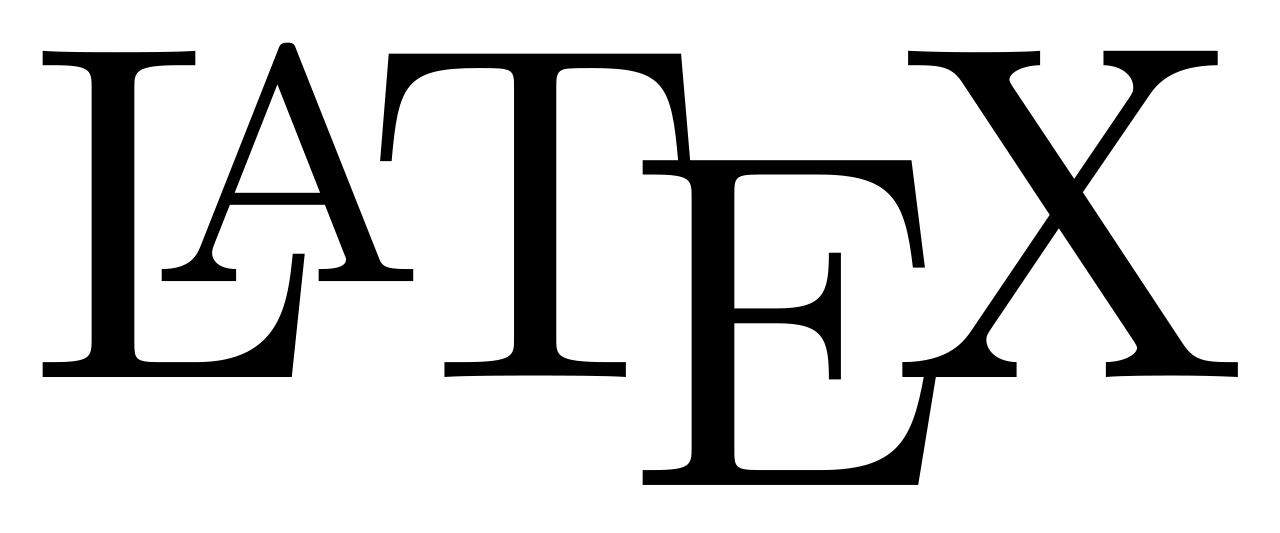
\includegraphics[scale=1]{latex-logo}
\end{lstlisting}
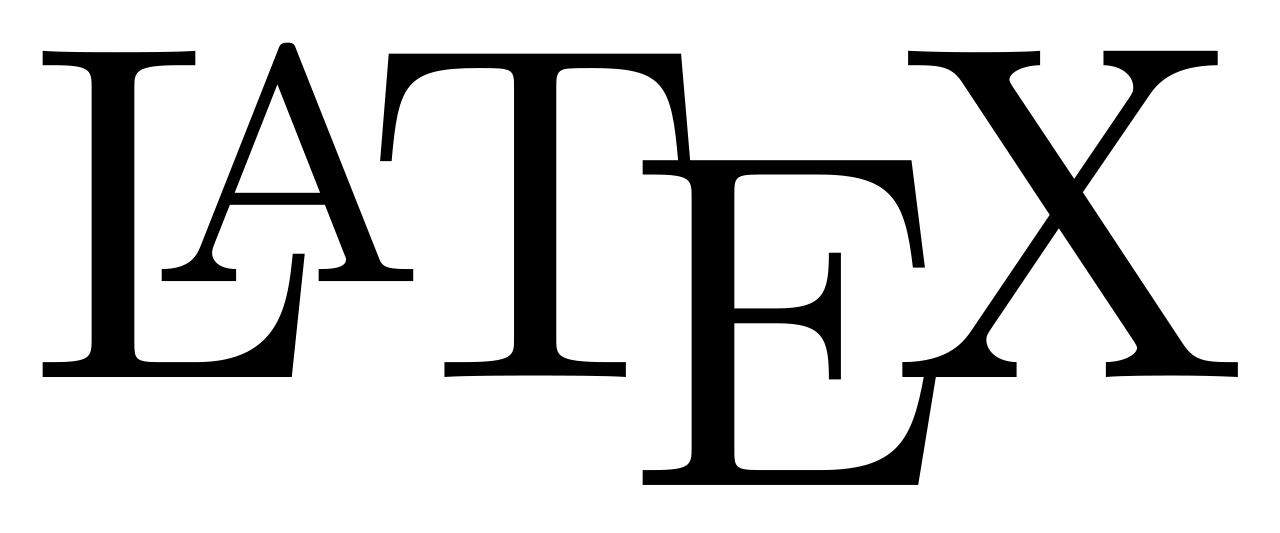
\includegraphics[scale=0.2]{latex-logo}

\lstset{language=Java}
\begin{lstlisting}
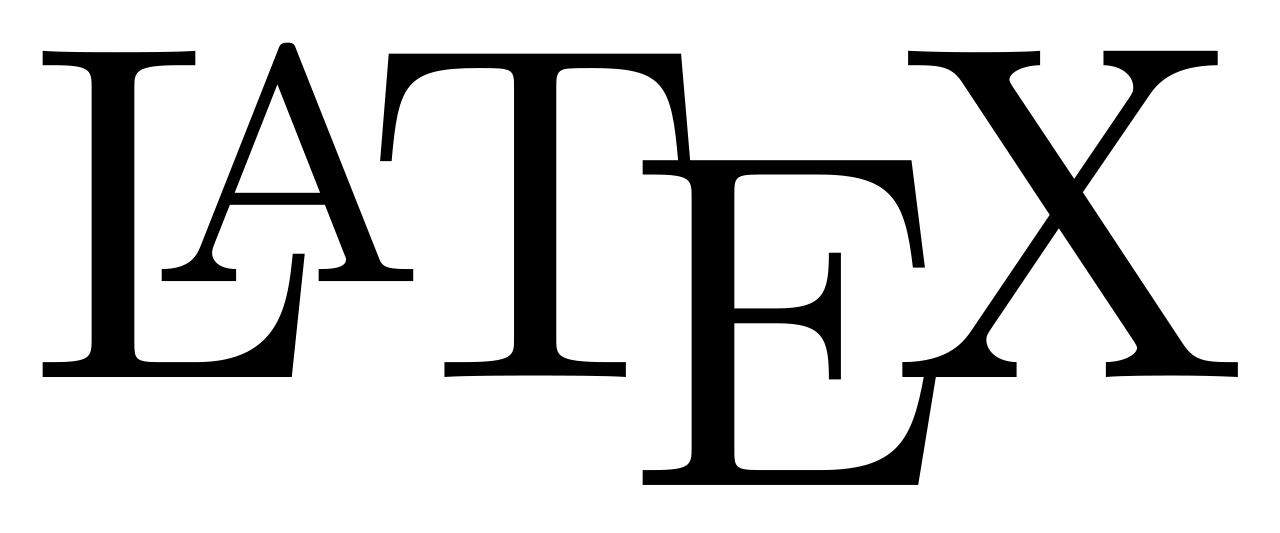
\includegraphics[width=3cm, height=4cm]{latex-logo}
\end{lstlisting}
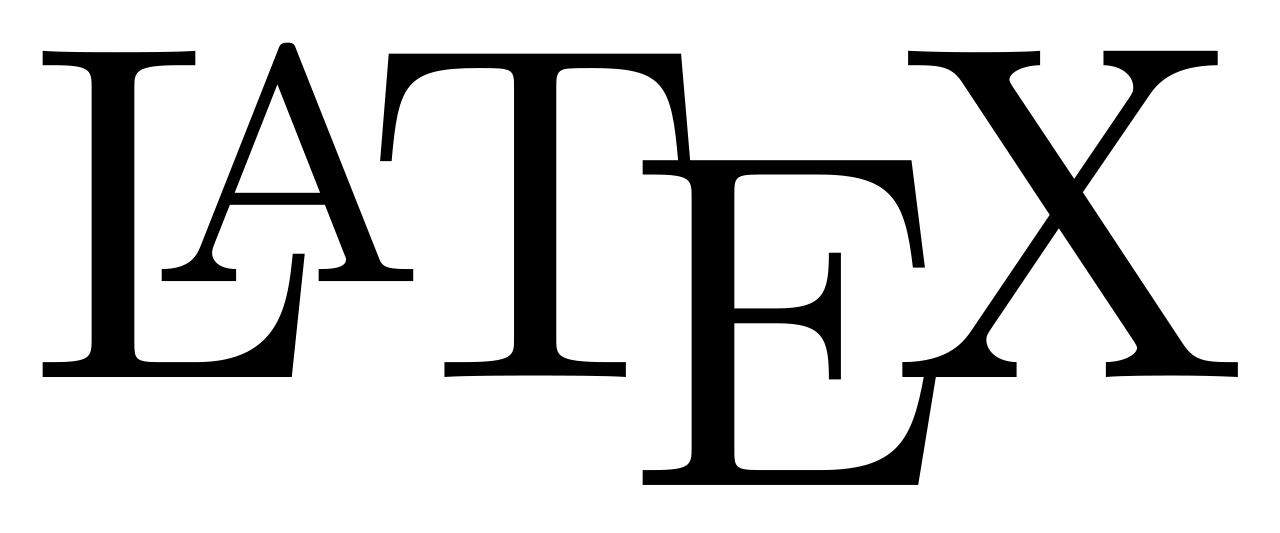
\includegraphics[width=3cm, height=4cm]{latex-logo}

\lstset{language=Java}
\begin{lstlisting}
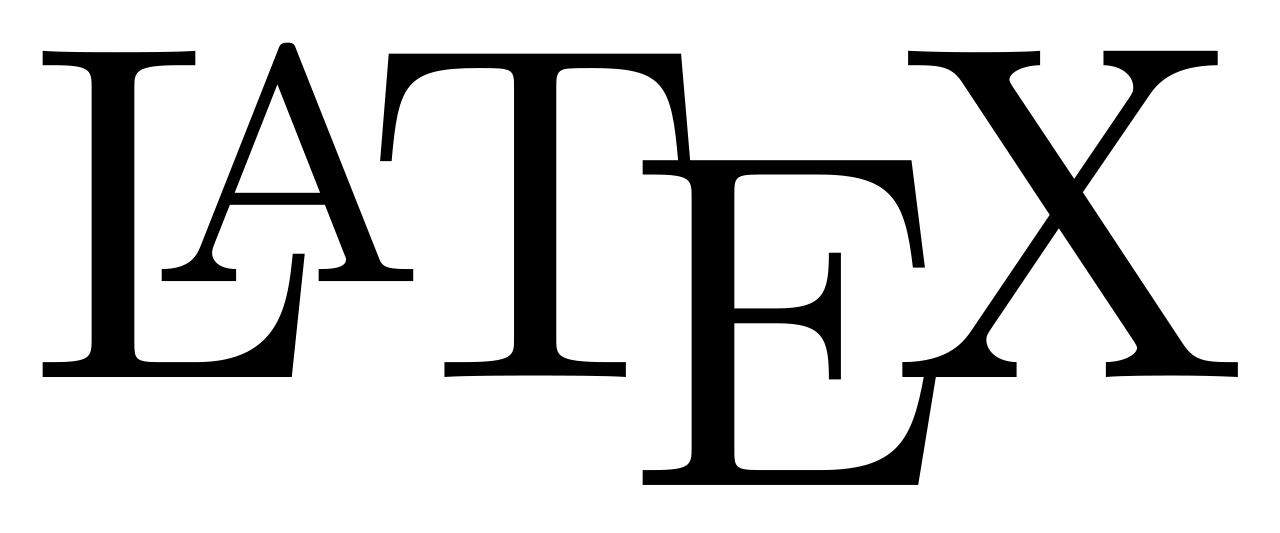
\includegraphics[width=\textwidth]{latex-logo}
\end{lstlisting}
Texto
\lstset{language=Java}
\begin{lstlisting}
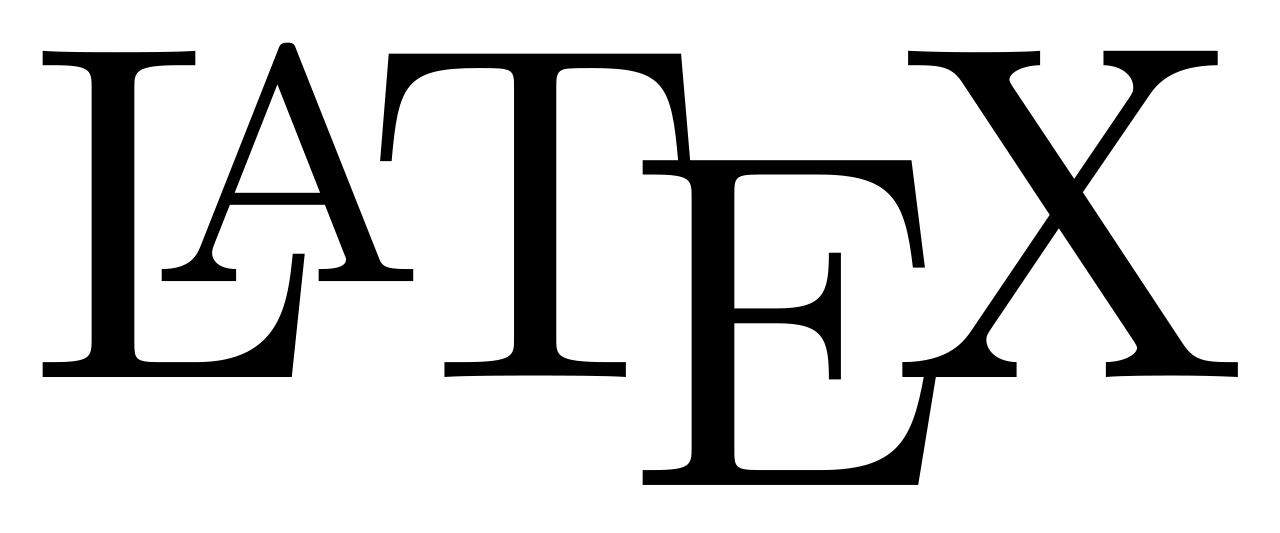
\includegraphics[scale=0.5, angle=45]{latex-logo}
\end{lstlisting}
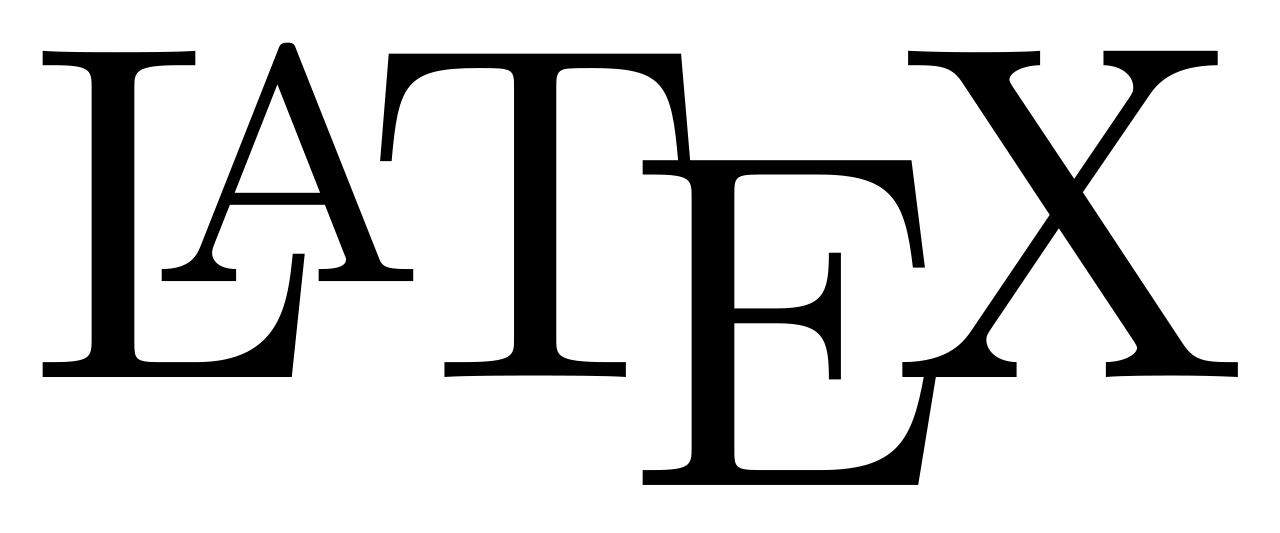
\includegraphics[scale=0.1, angle=45]{latex-logo}

\subsection{Posicionamiento}

\lstset{language=Java}
\begin{lstlisting}
\begin{figure}[posicionamiento]
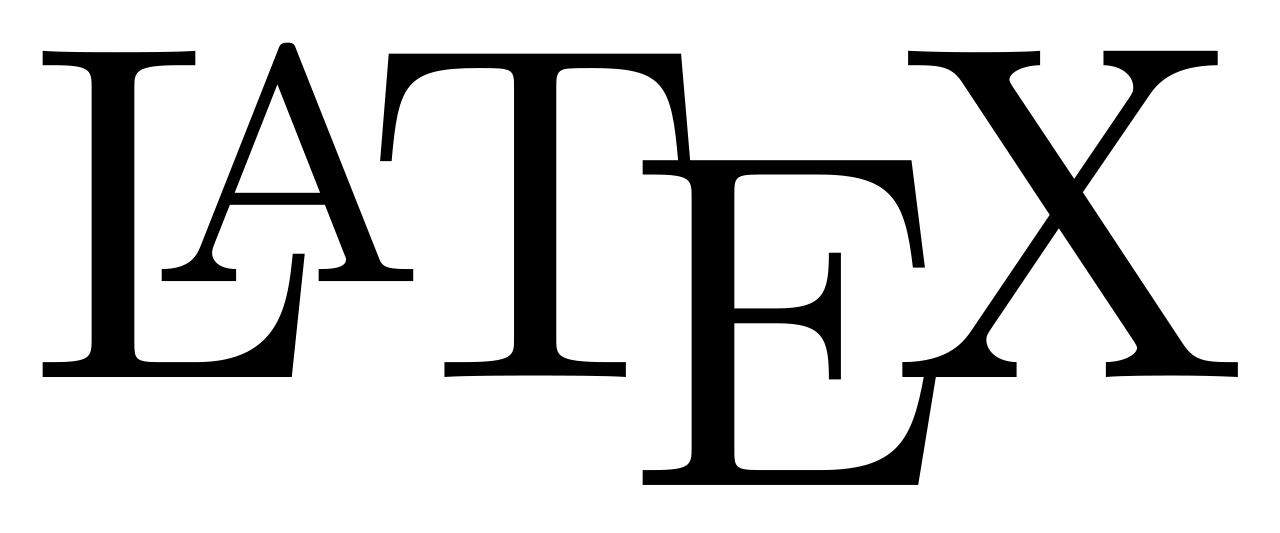
\includegraphics[width=8cm]{latex-logo}
\end{figure}
\end{lstlisting}

\begin{table}[H]
\centering
\resizebox{\textwidth}{!}{%
\begin{tabular}{cl}
\hline
\multicolumn{1}{l}{\textbf{Parámetro}} & \textbf{Posicionamiento}                                                                                                                                                                      \\ \hline
h                                      & \begin{tabular}[c]{@{}l@{}}Coloque el flotador aquí, es decir, aproximadamente en el mismo punto en el que \\ aparece el texto fuente (sin embargo, no exactamente en el punto).\end{tabular} \\ \hline
t                                      & Posición en la parte superior de la página.                                                                                                                                                   \\ \hline
b                                      & Posición en la parte inferior de la página.                                                                                                                                                   \\ \hline
p                                      & Se pone en una página especial para flotadores solamente.                                                                                                                                     \\ \hline
!                                      & Anula los parámetros internos que LaTeX esté utilizando.                                                                                                                                      \\ \hline
H                                      & \begin{tabular}[c]{@{}l@{}}Coloca el flotador exactamente en la ubicación del código LaTeX.\\  Requiere el paquete flotante. Esto es algo equivalente a h !.\end{tabular}                     \\ \hline
\end{tabular}%
}
\end{table}

\section{Manejo de figuras al lado de tablas (minipage)}
\subsection{Subsection 1}
Text here.

\section{Ecuaciones matem\'aticas}
\subsection{Subsection 1}
Text here.

\section{Manejo de colores}
\subsection{Subsection 1}
Text here.

\begin{thebibliography}{1}
\bibitem{paper1}A. Bryan  (2013) \emph{Vertical And Horizontal Privilege Escalation} [Blog post]. Retrieved from https://bryanavery.co.uk/vertical-and-horizontal-privilege-escalation/



\end{thebibliography}
\end{document}






